\section{Search, evidence preservation, and controls}
\label{sec:methods}

\subsection{Observations and search populations}

We searched public TESS photometry for recurring transit-like dimming
\cite{ricker2015}, using TESS-SPOC and Quick-Look Pipeline (QLP) products
\cite{caldwell2020,huang2020}. Target properties and initial contamination
estimates came from the TESS Input Catalog (TIC; \cite{tic2019}). The six
retained signals emerged from several successive, overlapping campaigns.
They are not six discoveries from a single uniform survey, and the denominators
in Table~\ref{tab:campaigns} must not be added to obtain a unique-star count.
The investigation was adaptive: later experiments responded to earlier
controls and candidate assessments. We report the executed selection and
its limitations rather than interpreting the final shortlist as a statistical
planet yield.

\begin{table}[htbp]
\centering
\small
\caption{Completed search scopes. Counts describe processing outcomes,
not astrophysical classifications. The weak-seed stars were already counted
in earlier searches; other scopes also overlap.}
\label{tab:campaigns}
\begin{tabularx}{\linewidth}{@{}l r X@{}}
\toprule
Scope & Attempts & Reconciled outcome \\
\midrule
Solar-radius pool & 7,004 & 4,481 below threshold; 2,494 flagged;
28 screening passes, all reviewed; one original data error. \\
Weak-seed refinement & 689 & 688 measurements and one error;
23 local flags, all reviewed; 22 deprioritized. \\
Faint QLP pilot & 100 & 46 below threshold; 54 flagged; no errors
or full screening passes. \\
Faint QLP expansion & 1,845 & 950 below threshold; 888 flagged;
seven original data failures. Six recoveries gave 1,844 usable searches;
17 peak follow-ups on 16 stars. \\
\bottomrule
\end{tabularx}
\end{table}

The solar-radius inventory selected catalog radii of
$0.81$--$1.10\,R_\odot$, TESS magnitudes $6$--$12$, and distances
up to 120~pc. Of 16,581 opportunities with early and later TESS-SPOC coverage,
408 were excluded by exact identifiers in saved planet, candidate, and
eclipsing-binary catalogs, 1,635 failed the contamination-ratio requirement
of at most 0.2 or lacked its value, and 7,534 lacked an adjacent early-sector
pair. The remaining 7,004 were ranked by
$R_\star^2 10^{0.2(T-10)}/\sqrt{N_{\rm train}}$.
This is a metadata-based noise proxy, not measured quietness.
The earliest contiguous group of two or three sectors numbered at most 55
trained discovery, while the latest available ordinary sector numbered
56--107 was reserved. No temperature cut was applied to this pool.

The fainter QLP pool used $12<T\leq13.5$, catalog radii
$0.15$--$0.5\,R_\odot$, distances up to 120~pc,
$T_{\rm eff}\leq4000$~K, and the same contamination-ratio limit.
Dated catalog exclusions, TIC quality dispositions, and prior raw-data
access were checked before selection. From 38,822 eligible metadata targets,
1,945 had a suitable four-sector sequence and a separate reserved epoch.
Discovery used the latest four consecutive QLP sectors ending no later
than sector 96; reserved sectors were at least eight sector numbers from
every training sector. Their actual training baseline could not exceed
120~days. Sector-number separation alone does not establish independent
or usable observations. The four-sector design followed limited known-planet
controls and was therefore an informed design change, not a blind survey
choice. The first 100 targets formed the pilot and the remaining 1,845 the
expansion. Six expansion failures were recovered with three usable assigned
sectors; one target remained unsearchable with only two. Recoveries are
neither additional stars nor equivalent to four-sector coverage.

\subsection{Preprocessing and recurring-dip search}

For TESS-SPOC we used corrected PDCSAP flux and its supplied errors.
We retained quality-zero samples with finite times and positive, finite fluxes
and uncertainties, sorted timestamps, and removed duplicate timestamps.
FITS identities, integrity information, raw-product URLs, retrieval records,
and SHA-256 hashes were retained. Times are expressed as
${\rm BTJD}={\rm BJD}_{\rm TDB}-2457000$.
QLP flux and error columns were recorded per product. Where a target's
explicitly enabled fallback encountered no usable published errors, it
assigned equal errors from the robust adjacent-difference scale,
$1.4826\,\operatorname{MAD}(\Delta f)/\sqrt{2}$.
This estimates short-timescale scatter rather than a calibrated correlated-noise
uncertainty. QLP discovery normally used inverse-variance 10-minute bins;
native sampling was retained for the solar-radius search and QLP refinements.

Each sector was divided at gaps longer than 0.3~days. We divided flux and
errors by a running-median trend with a 1.5-day window and repeated the
analysis with a 2.5-day window. Segments shorter than the filter window
or 30 samples were excluded, and half a window was trimmed from each edge.
Errors were floored at the robust first-difference scatter of the normalized
flux. Only extreme upward excursions, above eight such scatter units, were
removed; downward outliers were preserved. At least 200 clean samples were
required. These operations can attenuate or remove transits, especially near
gaps; a different reduction of the same exposures supplies a robustness
test, not independent photons.

The multi-sector search used Astropy box least squares (BLS;
\cite{kovacs2002,astropy2022}) with a likelihood objective, periods from
0.5~days to $\min(20\,{\rm days},B/2.5)$ for baseline $B$, and durations
$D=0.04$, 0.06, 0.09, 0.13, and 0.18~days. The BLS frequency factor was 2.
The ordinary dense-search baseline limit was 100~days, extended to
120~days for the four-sector QLP experiment. Up to three peaks separated
by more than 2\% in period were retained, including harmonics for later
inspection. Formal depth signal-to-noise ratio (SNR) of at least 7 triggered
diagnostics; a full screening pass required SNR at least 8 and all additional
gates below. Historical single-sector searches instead used periods
$0.7$--$\min(10,B/2.5)$~days, durations
0.06, 0.09, 0.13, 0.18, and 0.24~days, and frequency factor 0.8.

For a clock $(P,t_0,D)$, in-event samples satisfied
$|\phi|<D/2$ and local comparison samples
$D<|\phi|<\min(3D,P/2)$, where $\phi$ is the wrapped time offset.
Depth was the inverse-variance-weighted comparison mean minus the event
mean; its conditional variance was the sum of the two mean variances.
Measurements required at least two in-event and five comparison samples.
An event was supported when its formal depth SNR was at least 2.
Odd/even depths, a half-phase secondary, inverted-flux BLS, sinusoidal
variability, gap proximity, event consistency, and alternate detrending were
checked. These are heuristic screening diagnostics, not calibrated
false-alarm probabilities.

The weak-seed experiment revisited 689 below-threshold stars with at least
two unopened additional early sectors, retaining at most nine early sectors
and the original strongest peak as its sole seed. A local review flag
required SNR at least 8 under both detrendings, periods agreeing within
0.5\%, and neither timing profile touching its search boundary.
This was a restricted refinement, distinct from full-domain rediscovery
or a full screening pass.

\subsection{Frozen clocks and the holdout record}

Before testing reserved photometry, we recorded training inputs, the refined
clock, all accepted timing-profile pairs, and decision rules. Local refinement
tested durations $0.8D$, $D$, and $1.2D$, retaining period/epoch pairs within
$\Delta\log\mathcal{L}=4.5$ of the maximum, including disconnected islands.
The period half-width was $3DP/B_{\rm seed}$; grids contained at least
2,049 and at most 50,001 points. The epoch floor was
$\max(D/50,D/\max[\mathrm{SNR},1])$.
These are conditional box-model profiles with a heuristic floor, not
physical or correlated-noise confidence intervals.

We aligned profile epochs to a common cycle and propagated them to the
reserved observations. The maximum timing displacement plus three epoch
floors had to be less than $D/2$, the accepted profile could not reach
the period-grid boundary, and training required three supported events.
Recovery additionally required combined fixed-clock SNR at least 5 and
two supported reserved events. With adequate timing and expected formal
SNR at least 5, observed SNR below 2 constituted a non-recovery; insufficient
coverage, sensitivity, or timing otherwise remained inconclusive.
Fixed-period shifted-phase comparisons were dependent controls, not survey
false-alarm estimates. Refitted clocks, enlarged windows, alternate reductions,
and retrospective season omissions were retained as exploratory analyses;
already inspected observations did not become fresh holdouts.

One operational exception is material. TIC 5546257 sector 62 was opened
after its expanded-training prediction was frozen but before the parent
solar-radius queue's terminal audit. This violated that queue's reserved-cache
absence assertion. The queue stopped after ranks 3920--4431, the chronology
and raw-data hash were preserved in a supplemental audit, and the remaining
2,572 attempts resumed under a separate frozen plan. Original target records
and predictions were not overwritten. We therefore do not claim perfect
compliance with every original queue holdout rule. Later audits distinguish
historical pre-access cache checks from the subsequent opened-data state.

\subsection{Sensitivity and conditional reliability controls}

Table~\ref{tab:controls} includes unsuccessful controls as well as recoveries.
Five known shallow planets were selected before their photometry was opened,
using the solar-radius opportunity pool and catalog depth proxies near
200~ppm. Only Kepler-93~b and TOI-5159~b passed all gates.
TOI-1435~b was below threshold, TOI-5788~b failed SNR and detrending tests,
and variability obscured HD~63433~d. Recovery of the stronger TOI-5788~c
does not change the preselected-planet result of two out of five.
Figure~\ref{fig:known-controls} retains all five outcomes.

\begin{table}[htbp]
\centering
\small
\caption{Selected controls and their interpretation. These small, selected
experiments do not measure survey completeness or planet probabilities.}
\label{tab:controls}
\begin{tabularx}{\linewidth}{@{}l X X@{}}
\toprule
Experiment & Outcome & Principal limitation \\
\midrule
Known shallow planets & 2/5 preselected planets pass;
4/5 periods occur among the three retained peaks. &
Period recovery alone is not gate passage; nonrandom sample. \\
Raw-flux shallow injections & 3/18 recoveries at 100~ppm;
11/18 at 300~ppm, across three selected stars. &
One phase per configuration, box shapes, limited periods and durations. \\
TIC 469309982 permutations & 0/40 local-flag exceedances in each
of three block models. & Original target and seed selection are conditioned on. \\
TIC 96166003 permutations & 0/40 selected-family exceedances in each
of three block models. & Uses all already-opened sectors and a selected period family. \\
Deprioritized signals & TIC 362222987: 46/48 shuffled maxima
exceed the observation; TIC 396160833: 17/48. &
Conditional maximum-power comparisons, not physical classifications. \\
\bottomrule
\end{tabularx}
\end{table}

\begin{figure}[htbp]
\centering
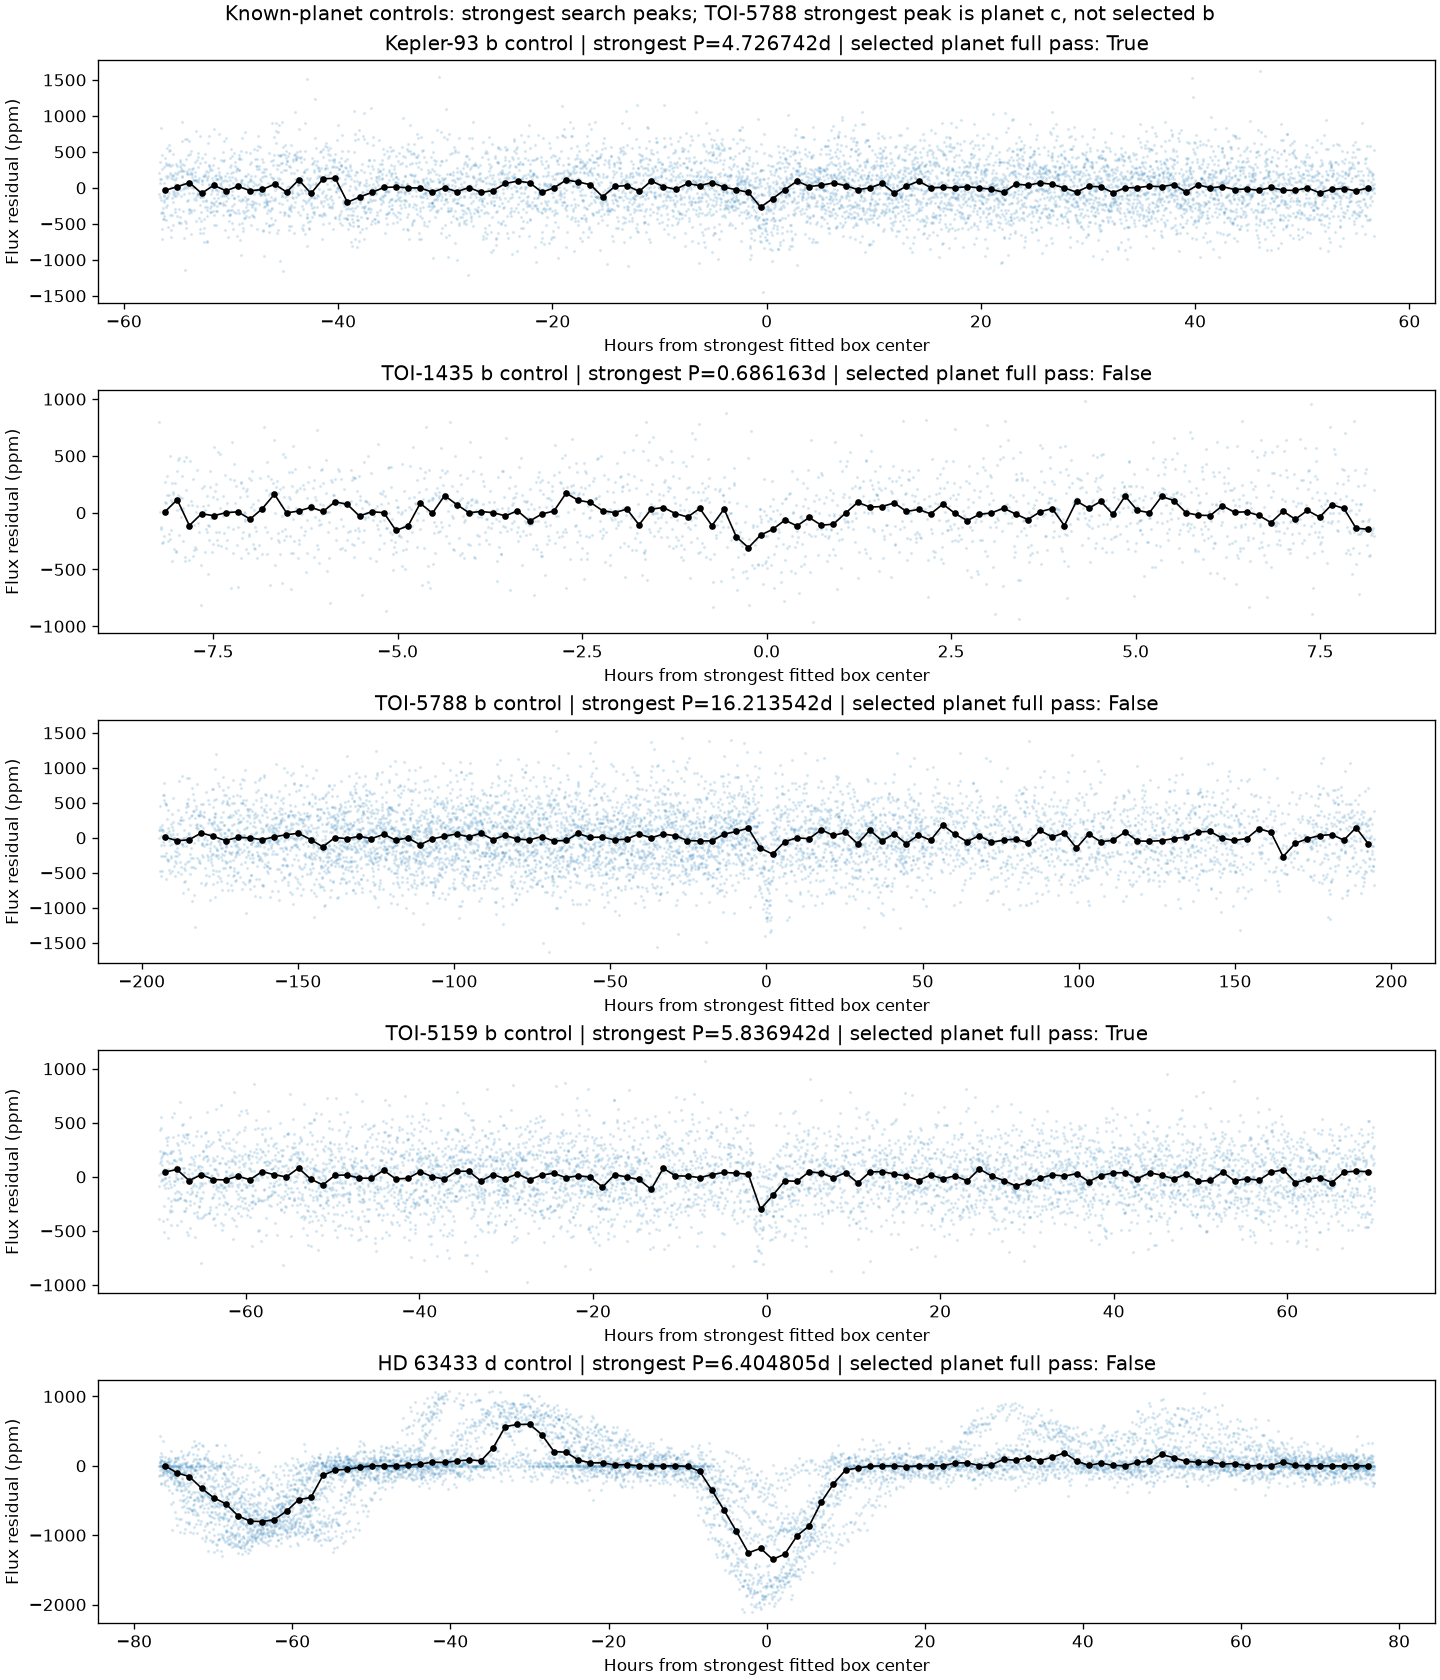
\includegraphics[width=\linewidth]{figures/controls-known.png}
\caption{Unchanged-pipeline searches of five preselected known planets.
The figure is retained from the archived control experiment. Successful
period agreement and full screening passage are different outcomes;
the two full passes do not establish population completeness.}
\label{fig:known-controls}
\end{figure}

The shallow-injection experiment applied exposure-integrated 100 and
300~ppm boxes to raw flux before detrending in three preselected
below-threshold targets. It tested periods 1.37, 4.73, and 13.13~days,
durations 0.04 and 0.12~days, and one phase per configuration.
All three 100-ppm recoveries occurred at the shortest period and longer
duration; none occurred at the two longer periods. Existing matching
baseline signals were not credited as recoveries. Thus negative searches
cannot exclude shallow planets on the basis of these examples.

For the two lower-priority signals in Table~\ref{tab:controls}, deterministic
0.25-, 0.5-, and 1-day blocks of paired raw flux and errors were permuted
within sector and gap-separated segments. Forty draws per model yielded
zero exceedances; each model's binomial 95\% Monte Carlo interval is
0--8.81\%. Counts were not pooled to claim a smaller bound.
Block seams, destroyed long correlations, retained signal fragments, and
unproven exchangeability limit interpretation. Four deterministic injections
for TIC 469309982 passed its local flag, but one selected a competing epoch
in one detrending; all four TIC 96166003 injections recovered the imposed
period and epoch. These checks verify processing behavior under selected
conditions, not the original search false-alarm probability.

\subsection{Attribution and uncertainty limitations}

Difference images compared mean local baseline and in-event pixels, with
propagated diagonal errors and inverse-variance event stacking. Conditional
source fits used mission response templates plus a planar background.
Neither fitted registration uncertainty nor response-model mismatch was
fully propagated into source rankings. Kepler-93~b exposes the practical
consequence: the target was preferred in sector 40, but a neighbor in
sector 41, despite a known shallow planetary signal. Stable rankings across
registration or event omissions can therefore accompany wrong attribution.

A separately frozen pointing-correction control passed three of four cases;
the contaminant's discrimination decreased in one sector. A template-free
paired-aperture diagnostic passed five of eight cases and preferred the wrong
Kepler-93 region twice. Neither met its gate for candidate application.
These failures prevent converting favorable candidate image fits into
calibrated host probabilities or using poor-model rankings alone to reject
a planet. Conditional circular, dark-occultor fits with exposure-integrated
\texttt{batman} models \cite{kreidberg2015} likewise assess compatibility
under assumed hosts and dilution; they do not exclude stellar companions.

Time-averaging audits of the two strongest signals follow the correlated-noise
rationale of \cite{pont2006}. They retain adverse event omissions and
insufficient-bin cases, but use different estimators: one compares fitted
residual bins with simulated white-noise refits, while the other examines
out-of-event bins. Their scalar error inflation is a sensitivity analysis,
not a complete covariance model or interchangeable reliability score.
Agreement between reductions sharing photons, successful arithmetic
verification, and conditional astrophysical scenario weights do not provide
independent observations or validation \cite{giacalone2021}.

\subsection{Detailed full-screen rejection gates}
\label{sec:screen-gates}

For reproducibility, a full-screen peak was flagged for any of the following:
formal SNR below 8; fewer than three supported events; an unmeasurable
odd/even comparison or discrepancy above $3\sigma$; an unmeasurable
half-phase secondary or secondary SNR above 3; inverted-to-original
maximum BLS power ratio at least 0.8; sinusoidal likelihood improvement
greater than the box improvement; or duty cycle $D/P>0.15$.
Additional flags applied when duration-binned correlated noise was
unmeasurable or reduced SNR below 7, event-depth consistency had conditional
chi-square survival below 0.001, one event contributed more than 75\%
of summed positive event SNR squared, or more than half the supported
events lay within $\max(0.15\,{\rm days},D)$ of a clean-segment edge.
The alternate detrending's strongest period had to agree within 2\%,
and every supplied aperture crowding fraction had to be at least 0.8.
Missing crowding information remained a flag, including for QLP products;
separately labeled diagnostic-only follow-ups did not erase original failures.
The discovery noise ratio used robust scatter of out-of-event duration-bin
means relative to their expected white errors, with a floor of one,
at least 15 bins, and at least half the expected sampling in each bin.
These exact numerical gates define the experiment; they do not constitute
an empirically calibrated planet classifier.
